\documentclass[11pt,a4paper]{article}

\usepackage[margin=2.5cm]{geometry}
\usepackage{amsmath,amssymb}
\usepackage{booktabs}
\usepackage{longtable}
\usepackage{array}
\usepackage{graphicx}
\usepackage{caption}
\usepackage{enumitem}
\usepackage{xcolor}
\usepackage{hyperref}
\usepackage{listings}
\usepackage{tikz}
\usetikzlibrary{arrows.meta,positioning,shapes.geometric}

\hypersetup{
  colorlinks=true,
  linkcolor=blue!60!black,
  citecolor=blue!60!black,
  urlcolor=blue!60!black,
}

\lstset{
  basicstyle=\ttfamily\small,
  breaklines=true,
  frame=single,
  columns=fullflexible,
  keepspaces=true,
  showstringspaces=false,
}

\newcommand{\repo}[1]{\texttt{#1}}
\newcommand{\note}[1]{\textit{Note:}~#1}

\title{Reproducing the UIT-VSMEC Stacked Ensemble\\for Vietnamese Emotion Recognition}
\author{}
\date{}

\begin{document}
\maketitle

\begin{abstract}
This document provides a self-contained reproduction guide for the Vietnamese fine-grained emotion recognition pipeline implemented in the \repo{topicmodeling} repository. The workflow begins with retrieval of the UIT-VSMEC corpus, applies LLM data augmentation on the raw training split, then runs Vietnamese text preprocessing on all splits, and culminates in a three-tier stacked ensemble: five heterogeneous base classifiers produce out-of-fold probability estimates; a stacking layer constructs structured meta-examples with validation-accuracy weights; and a QLoRA-adapted Gemma-2-9B-it meta-model learns to emit the final emotion label. All steps are designed for execution on Google Colab with CUDA GPUs (A100, T4, or G4) in high-RAM mode. Successful reproduction is confirmed by the presence of \repo{tm\_research/ensemble/artifacts/metrics/ensemble\_summary.json}, which reports test-set accuracy of approximately 0.7023 and weighted F1 of approximately 0.7022 for the full system.
\end{abstract}

\noindent\textbf{Keywords:} UIT-VSMEC, Vietnamese emotion recognition, stacked ensemble, QLoRA, Gemma, data augmentation, reproduction guide

\section{Introduction}
\label{sec:intro}

The objective of this work is to improve macro-level and minority-class performance on Vietnamese social-media emotion classification by combining heterogeneous base models with an LLM-based meta-learner. The corpus is UIT-VSMEC (Vietnamese Social Media Emotion Corpus), a seven-class dataset with labels \texttt{Enjoyment}, \texttt{Sadness}, \texttt{Fear}, \texttt{Anger}, \texttt{Disgust}, \texttt{Surprise}, and \texttt{Other}. Each instance consists of a Vietnamese sentence (\texttt{text}) and an emotion category (\texttt{label}).

The canonical inputs for the ensemble framework are three processed CSV files under \repo{tm\_research/data/processed/}:
\begin{itemize}[nosep]
  \item \repo{train\_1500\_final.csv} --- augmented and cleaned training split;
  \item \repo{val\_final.csv} --- validation split;
  \item \repo{test\_final.csv} --- held-out test split.
\end{itemize}
The loader in \repo{tm\_research/ensemble/utils\_io.py} normalizes column names automatically: text is read from \texttt{Sentence\_clean}, \texttt{Sentence}, or \texttt{text}; labels are read from \texttt{Emotion} or \texttt{label}. Labels are mapped to integer identifiers in alphabetical order and persisted to \repo{artifacts/label\_map.json}.

This guide covers four stages: (1)~data retrieval, (2)~LLM data augmentation, (3)~text preprocessing, and (4)~the stacked ensemble (notebooks 01--07). Standalone BERT experiments, machine-learning baselines, and the auxiliary topic-modeling CLI are out of scope.

\section{Computational Environment}
\label{sec:environment}

\subsection{Google Colab Requirements}

The pipeline was developed and executed primarily on Google Colab with GPU acceleration and high-RAM runtimes. Table~\ref{tab:hardware} summarizes the hardware requirements.

\begin{table}[htbp]
  \centering
  \caption{Global hardware requirements for Google Colab.}
  \label{tab:hardware}
  \begin{tabular}{@{}ll@{}}
    \toprule
    Resource & Requirement \\
    \midrule
    GPU & CUDA-enabled: A100 (preferred), T4, or G4 \\
    System RAM & High-RAM mode; 22--80\,GB depending on runtime \\
    Notebook 06 peak RAM & Approximately 80\,GB \\
    VRAM (notebooks 06--07) & Approximately 24\,GB (4-bit QLoRA on Gemma-2-9B-it) \\
    Storage & Google Drive mount recommended for artifact persistence \\
    \bottomrule
  \end{tabular}
\end{table}

\begin{table}[htbp]
  \centering
  \caption{Per-notebook resource requirements.}
  \label{tab:notebook-resources}
  \small
  \begin{tabular}{@{}llll@{}}
    \toprule
    Notebook & GPU & RAM (approx.) & Notes \\
    \midrule
    \repo{Data\_Augmentation\_LLM.ipynb} & Optional & Low & API-bound \\
    \repo{DataPreprocessing.ipynb} & Optional & Low & CPU sufficient \\
    \repo{ensemble/01}--\repo{04} & Required & 22--40\,GB & 3-fold OOF, 20 epochs each \\
    \repo{ensemble/05} & Optional & Low & Builds JSONL meta-dataset \\
    \repo{ensemble/06} & Required & $\sim$80\,GB & QLoRA meta-model training \\
    \repo{ensemble/07} & Required & 40--80\,GB & Inference and baseline comparison \\
    \bottomrule
  \end{tabular}
\end{table}

\subsection{Repository Setup on Colab}

\begin{enumerate}[label=\arabic*.]
  \item Clone or upload the repository to Google Drive. The default path used in ensemble notebooks is:
  \begin{lstlisting}
/content/drive/MyDrive/thesis/topicmodeling
  \end{lstlisting}
  \item In Colab, select \emph{Runtime $\rightarrow$ Change runtime type}, enable a GPU (A100 when available), and turn on \emph{High-RAM}.
  \item Mount Google Drive and configure ephemeral scratch space. Each ensemble notebook begins with a setup cell that calls \repo{setup\_colab()} from \repo{tm\_research/ensemble/colab\_setup.py}:
  \begin{lstlisting}
import os, sys
REPO_ROOT = '/content/drive/MyDrive/thesis/topicmodeling'
TMP_ROOT = '/content/ensemble_tmp'

if 'google.colab' in sys.modules:
    from google.colab import drive
    if not os.path.ismount('/content/drive'):
        drive.mount('/content/drive')
    if REPO_ROOT not in sys.path:
        sys.path.insert(0, REPO_ROOT)

from tm_research.ensemble.colab_setup import setup_colab
paths = setup_colab(repo_root=REPO_ROOT, tmp_root=TMP_ROOT)
  \end{lstlisting}
  This mounts Drive, routes HuggingFace cache and trainer checkpoints to \repo{/content/ensemble\_tmp}, and copies prior artifacts from Drive when resuming a session.
  \item After each ensemble notebook completes, persist artifacts to Drive:
  \begin{lstlisting}
from tm_research.ensemble.utils_io import push_artifacts_to_persistent
push_artifacts_to_persistent()
  \end{lstlisting}
\end{enumerate}

\subsection{API Keys and Secrets}

\begin{table}[htbp]
  \centering
  \caption{Required credentials.}
  \label{tab:secrets}
  \begin{tabular}{@{}lll@{}}
    \toprule
    Variable & Used by & Configuration \\
    \midrule
    \texttt{GOOGLE\_API\_KEY} & LLM augmentation & Colab Secret or \repo{tm\_research/.env} \\
    \texttt{HF\_TOKEN} & Gemma-2 download & Colab Secret; accept Gemma-2 license on HuggingFace \\
    \bottomrule
  \end{tabular}
\end{table}

For \texttt{HF\_TOKEN}, create a token at \url{https://huggingface.co/settings/tokens} and accept the license at \url{https://huggingface.co/google/gemma-2-9b-it}. In Colab, add the token via the key icon in the sidebar (\emph{Secrets}) and grant notebook access.

\subsection{Software Dependencies}

Install Python dependencies from the repository root:
\begin{lstlisting}
pip install -r requirements.txt
\end{lstlisting}
Ensemble notebooks additionally install, via \texttt{\%pip install}:
\texttt{torchao}, \texttt{peft}, \texttt{trl}, \texttt{bitsandbytes}, \texttt{accelerate}, \texttt{transformers}, and \texttt{datasets}.

\section{End-to-End Pipeline Overview}
\label{sec:overview}

Figure~\ref{fig:pipeline} depicts the complete workflow from raw data to ensemble evaluation.

\begin{figure}[htbp]
  \centering
  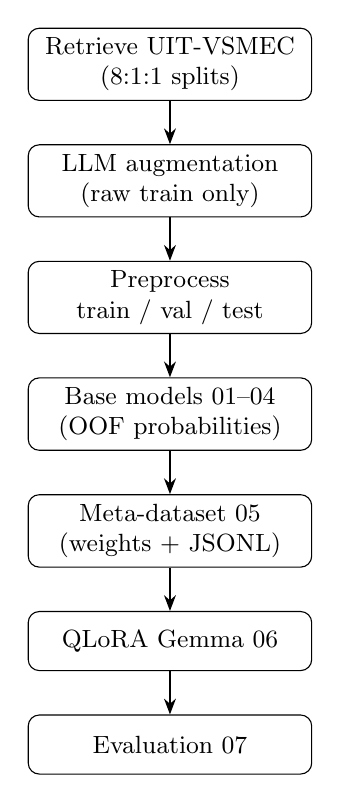
\begin{tikzpicture}[
    node distance=0.55cm and 0.4cm,
    box/.style={draw, rounded corners, align=center, minimum width=3.6cm,
                minimum height=0.75cm, font=\small},
    arr/.style={-{Stealth[length=2mm]}, thick}
  ]
    \node[box] (retrieve) {Retrieve UIT-VSMEC\\(8:1:1 splits)};
    \node[box, below=of retrieve] (augment) {LLM augmentation\\(raw train only)};
    \node[box, below=of augment] (preprocess) {Preprocess\\train / val / test};
    \node[box, below=of preprocess] (base) {Base models 01--04\\(OOF probabilities)};
    \node[box, below=of base] (meta) {Meta-dataset 05\\(weights + JSONL)};
    \node[box, below=of meta] (lora) {QLoRA Gemma 06};
    \node[box, below=of lora] (eval) {Evaluation 07};
    \foreach \a/\b in {retrieve/augment, augment/preprocess,
                       preprocess/base, base/meta, meta/lora, lora/eval}
      \draw[arr] (\a) -- (\b);
  \end{tikzpicture}
  \caption{End-to-end reproduction pipeline for the UIT-VSMEC stacked ensemble.}
  \label{fig:pipeline}
\end{figure}

The minimum path to reproduce the headline ensemble result requires Stages~1--3 (data retrieval, augmentation on raw train, preprocessing of all splits) and Stage~4 (notebooks 01--07 run sequentially on a GPU machine).

\section{Stage 1: Data Retrieval}
\label{sec:retrieval}

\subsection{Objective}
Obtain the official UIT-VSMEC train, validation, and test splits and place them in the repository in a form ready for augmentation and preprocessing.

\subsection{Data Sources}
The corpus may be obtained from either of the following sources:
\begin{itemize}[nosep]
  \item Official release: \url{https://nlp.uit.edu.vn/datasets}
  \item HuggingFace mirror: \url{https://huggingface.co/datasets/tridm/UIT-VSMEC}
\end{itemize}

\subsection{Required Raw Files}
Place the following Excel files under \repo{data/} at the repository root (not committed to git):
\begin{itemize}[nosep]
  \item \repo{train\_nor\_811.xlsx} --- training split (approximately 5{,}548 rows after ID removal);
  \item \repo{valid\_nor\_811.xlsx} --- validation split (approximately 686 rows);
  \item \repo{test\_nor\_811.xlsx} --- test split (approximately 693 rows).
\end{itemize}
The suffix \texttt{811} denotes the standard 80\%/10\%/10\% split ratio used throughout the project.

\subsection{Procedure}
The loading procedure follows \repo{tm\_research/EmoModel\_Local.ipynb}:
\begin{enumerate}[label=\arabic*.]
  \item Load each Excel file with \texttt{pandas.read\_excel}.
  \item Drop the first column, which contains record identifiers not used in modeling.
  \item Retain at minimum the columns \texttt{Emotion} and \texttt{Sentence}. If present, retain \texttt{emotion\_vn} (Vietnamese emotion descriptor).
  \item Do \emph{not} reshuffle or merge the official splits; deduplication and shuffling are applied only during preprocessing (Stage~3) and only within each split.
\end{enumerate}

\subsection{Verification}
Confirm that the three files exist under \repo{data/} and that each dataframe contains non-null \texttt{Emotion} and \texttt{Sentence} fields with seven distinct emotion labels. The training split is ready for Stage~2 augmentation without any text cleaning.

\section{Stage 2: LLM Data Augmentation}
\label{sec:augmentation}

\subsection{Objective}
Balance the training set by generating synthetic Vietnamese social-media sentences for under-represented emotion classes on \emph{raw} training text, thereby improving minority-class recall in downstream models.

\subsection{Inputs and Configuration}
\begin{table}[htbp]
  \centering
  \caption{LLM augmentation configuration.}
  \label{tab:augmentation}
  \begin{tabular}{@{}ll@{}}
    \toprule
    Item & Value \\
    \midrule
    Notebook & \repo{tm\_research/Data\_Augmentation\_LLM.ipynb} \\
    Input & \repo{data/train\_nor\_811.xlsx} (raw train split; ID column removed) \\
    LLM & \texttt{gemini-2.5-flash} via LangChain \texttt{ChatGoogleGenerativeAI} \\
    API key & \texttt{GOOGLE\_API\_KEY} \\
    Target per class & \texttt{target\_per\_emotion=1500} \\
    Few-shot examples & 10 per class, sampled with replacement \\
    Temperature & 0.7 (default in augmenter class) \\
    \bottomrule
  \end{tabular}
\end{table}

\note{Augmentation must operate on raw \texttt{Sentence} text. If a \texttt{Sentence\_clean} column is present, drop it before generation. The Colab setup cell in the notebook loads Excel directly from Drive; locally, \texttt{pandas.read\_excel} on \repo{train\_nor\_811.xlsx} after dropping the ID column is equivalent.}

\subsection{Procedure}
\begin{enumerate}[label=\arabic*.]
  \item Set \texttt{GOOGLE\_API\_KEY} in \repo{tm\_research/.env} or as a Colab Secret.
  \item Open \repo{Data\_Augmentation\_LLM.ipynb} and load the raw training split:
  \begin{lstlisting}
import pandas as pd
df_train = pd.read_excel('data/train_nor_811.xlsx')
df_train = df_train.drop(df_train.columns[0], axis=1)
if 'Sentence_clean' in df_train.columns:
    df_train = df_train.drop('Sentence_clean', axis=1)
  \end{lstlisting}
  \item Initialize \texttt{BatchEmotionAugmenterLangChain} with the Gemini model.
  \item Call \texttt{run\_balanced\_augmentation()} with \texttt{target\_per\_emotion=1500}. For each emotion class below the target, the function computes the deficit, schedules async batch generation calls, and trims output to the exact number of samples needed.
  \item Merge synthetic rows with originals via \texttt{combine\_with\_original()}, tagging provenance columns (\texttt{augmented}, \texttt{source}, \texttt{source\_example\_idx}, \texttt{source\_example}).
  \item Apply the label normalization fix: replace \texttt{buon ba} with \texttt{buon} in the \texttt{emotion\_vn} column.
  \item Export the balanced dataset to \repo{tm\_research/data/processed/}.
\end{enumerate}

\subsection{Outputs}
\begin{table}[htbp]
  \centering
  \caption{Augmentation outputs (Stage~2).}
  \label{tab:augmentation-outputs}
  \begin{tabular}{@{}ll@{}}
    \toprule
    File & Description \\
    \midrule
    \repo{train\_balanced\_optimized.csv} & Original and synthetic rows with full provenance \\
    \repo{train\_1500\_gen\_eval.csv} & Evaluation export with trace columns ($\sim$10{,}558 rows) \\
    \repo{train\_1500\_gen\_clean.csv} & Training-ready export (\texttt{Emotion}, \texttt{Sentence}, \texttt{emotion\_vn}) \\
    \bottomrule
  \end{tabular}
\end{table}

Optional quality assurance may be performed with \repo{Synthetic\_Data\_Fidelity\_Eval.ipynb}; this step is not required for ensemble reproduction.

\subsection{Verification}
Inspect the emotion distribution in \repo{train\_1500\_gen\_clean.csv}. Each of the seven classes should contain approximately 1{,}500 samples (Enjoyment may retain slightly more originals, e.g., 1{,}558). Confirm zero missing values before proceeding to Stage~3.

\section{Stage 3: Text Preprocessing}
\label{sec:preprocessing}

\subsection{Objective}
Transform raw and augmented Vietnamese social-media text into clean, model-ready CSV files for ensemble training. Preprocessing runs \emph{after} augmentation on the combined train set, and on the raw validation and test splits.

\subsection{Shared Preprocessing Logic}
All cleaning is implemented in \repo{tm\_research/text\_preprocess.py} via the function \texttt{preprocess\_vietnamese\_text(text)}. The pipeline applies the following transformations in sequence:
\begin{enumerate}[label=\arabic*.]
  \item \textbf{Emoji replacement.} A dictionary of 116 emoji-to-Vietnamese mappings converts Unicode emoji into descriptive Vietnamese words (e.g., ``vui ve'' for happy, ``buon ba'' for sad, ``tuc gian'' for angry). Remaining emoji are stripped by a comprehensive Unicode regex.
  \item \textbf{Text emoticon replacement.} Thirty-nine text emoticon patterns (sorted longest-first to avoid partial matches) are mapped to Vietnamese descriptors (e.g., the emoticon \lstinline|:))| maps to ``cuoi lon'', meaning loud laughter).
  \item \textbf{Abbreviation expansion.} Ninety-five Vietnamese internet abbreviations are expanded via exact word-level matching (e.g., \texttt{ko} maps to ``khong'', meaning no/not).
  \item \textbf{Special character cleaning.} URLs, HTML tags, and non-Vietnamese characters are removed or normalized; repeated punctuation is collapsed; excess whitespace is trimmed; text is lowercased.
  \item \textbf{Deduplication.} Duplicate sentences are removed based on the cleaned text column, keeping the first occurrence only \emph{within each split}.
\end{enumerate}

\note{Stopwords are intentionally \emph{not} removed. BERT-based models rely on self-attention over all tokens; function words such as \emph{khong} (negation) and \emph{rat} (very) carry critical emotion signals.}

\subsection{Procedure}
Run \repo{DataPreprocessing.ipynb} once per split, setting \texttt{INPUT\_FILE} and \texttt{OUTPUT\_FILE} as follows:

\begin{table}[htbp]
  \centering
  \caption{Preprocessing runs (Stage~3).}
  \label{tab:preprocess-runs}
  \begin{tabular}{@{}lll@{}}
    \toprule
    Split & Input & Output \\
    \midrule
    Train & \repo{train\_1500\_gen\_clean.csv} & \repo{train\_1500\_final.csv} \\
    Validation & \repo{valid\_nor\_811.xlsx} (via CSV export) & \repo{val\_final.csv} \\
    Test & \repo{test\_nor\_811.xlsx} (via CSV export) & \repo{test\_final.csv} \\
    \bottomrule
  \end{tabular}
\end{table}

For each run, the notebook loads the input, applies \texttt{preprocess\_vietnamese\_text()} to the \texttt{Sentence} column (stored as \texttt{Sentence\_clean}), removes empty rows, deduplicates within the split, shuffles with random seed~42, and exports the result.

\textbf{Training split.} Set \texttt{INPUT\_FILE} to \repo{train\_1500\_gen\_clean.csv} and \texttt{OUTPUT\_FILE} to \repo{train\_1500\_final.csv}.

\textbf{Validation and test splits.} Load the Excel file from Stage~1, drop the ID column, export a temporary CSV if needed, then run the same cleaning pass. Reference pattern for validation:
\begin{lstlisting}
import pandas as pd
from tm_research.text_preprocess import preprocess_vietnamese_text

df = pd.read_excel('data/valid_nor_811.xlsx')
df = df.drop(df.columns[0], axis=1)
df['Sentence_clean'] = df['Sentence'].apply(preprocess_vietnamese_text)
df = df[df['Sentence_clean'].str.strip() != ''].drop_duplicates(
    subset='Sentence_clean', keep='first')
df = df.sample(frac=1, random_state=42).reset_index(drop=True)
df.to_csv('tm_research/data/processed/val_final.csv', index=False)
\end{lstlisting}
Repeat for \repo{test\_nor\_811.xlsx} $\rightarrow$ \repo{test\_final.csv}, or use \repo{DataPreprocessing.ipynb} with the corresponding paths.

\subsection{Canonical Ensemble Outputs}
\begin{table}[htbp]
  \centering
  \caption{Canonical ensemble CSV files (Stage~3 outputs).}
  \label{tab:final-csv}
  \begin{tabular}{@{}ll@{}}
    \toprule
    File & Derivation \\
    \midrule
    \repo{train\_1500\_final.csv} & \repo{train\_1500\_gen\_clean.csv} via \repo{DataPreprocessing.ipynb} \\
    \repo{val\_final.csv} & Raw validation Excel via same cleaning pipeline \\
    \repo{test\_final.csv} & Raw test Excel via same cleaning pipeline \\
    \bottomrule
  \end{tabular}
\end{table}

\subsection{Verification}
After completing Stage~3, confirm:
\begin{itemize}[nosep]
  \item \repo{train\_1500\_final.csv} contains approximately 10{,}541 cleaned records (post-deduplication of augmented data);
  \item \repo{val\_final.csv} and \repo{test\_final.csv} contain approximately 686 and 693 records respectively;
  \item All seven emotion labels are present in each split;
  \item The \texttt{Sentence\_clean} column is populated for ensemble loading.
\end{itemize}

\section{Stage 4: Stacked Ensemble Framework}
\label{sec:ensemble}

\note{Run Stage~4 only after Stage~3 has produced \repo{train\_1500\_final.csv}, \repo{val\_final.csv}, and \repo{test\_final.csv}.}

\subsection{Architecture Overview}
The ensemble comprises three tiers (see \repo{tm\_research/ensemble/WORKFLOW.md}):

\begin{enumerate}[label=\arabic*.]
  \item \textbf{Base model tier} (notebooks 01--04). Five heterogeneous classifiers---PhoBERT, CafeBERT, ViBERT, Logistic Regression, and Linear SVC---each produce soft probability vectors for every training, validation, and test instance. BERT models use 3-fold stratified out-of-fold (OOF) training; sklearn models share a TF-IDF pipeline.
  \item \textbf{Stacking tier} (notebook 05). Validation accuracies determine per-model weights $w_i = \mathrm{acc}_i / \sum_j \mathrm{acc}_j$. Structured prompts combining the input text, weighted-average probabilities, and per-model probability stacks are written to JSONL files.
  \item \textbf{Meta-model tier} (notebooks 06--07). Gemma-2-9B-it is fine-tuned with QLoRA on the JSONL meta-dataset. The model learns to output \texttt{<label>EMOTION</label>} given the structured prompt. Evaluation compares the LoRA-adapted meta-model against weighted-average and single-model baselines.
\end{enumerate}

\subsection{Out-of-Fold Protocol}
To prevent information leakage into the meta-training set:
\begin{itemize}[nosep]
  \item During OOF generation, each training instance receives probability estimates from a model that was \emph{not} trained on that instance.
  \item After OOF completion, each base model is retrained on the full training set and used to predict validation and test probabilities.
  \item Meta-dataset rows for \textbf{train} use OOF probabilities; rows for \textbf{val} and \textbf{test} use full-train-refit probabilities.
\end{itemize}

\subsection{Notebook Execution Guide}
Run the following notebooks \emph{in order} under \repo{tm\_research/ensemble/}. Each notebook's first cells call \repo{setup\_colab()}; the final cell should call \repo{push\_artifacts\_to\_persistent()}.

\begin{table}[htbp]
  \centering
  \caption{Ensemble notebook execution sequence.}
  \label{tab:ensemble-notebooks}
  \small
  \begin{tabular}{@{}clll@{}}
    \toprule
    Step & Notebook & Model / action & Artifacts \\
    \midrule
    01 & \repo{01\_base\_phobert\_oof.ipynb} & \texttt{vinai/phobert-base-v2} & \repo{probs/phobert\_\{oof,val,test\}.npy} \\
    02 & \repo{02\_base\_cafebert\_oof.ipynb} & \texttt{uitnlp/CafeBERT} & \repo{probs/cafebert\_*.npy} \\
    03 & \repo{03\_base\_vibert\_oof.ipynb} & \texttt{FPTAI/vibert-base-cased} & \repo{probs/vibert\_*.npy} \\
    04 & \repo{04\_base\_sklearn\_oof.ipynb} & TF-IDF + LogReg + LinearSVC & \repo{probs/logreg\_*.npy}, \repo{svc\_*.npy} \\
    05 & \repo{05\_weights\_and\_meta\_dataset.ipynb} & Weight computation + JSONL & \repo{weights.json}, \repo{meta\_jsonl/} \\
    06 & \repo{06\_train\_meta\_lora\_gemma.ipynb} & QLoRA on Gemma-2-9B-it & \repo{lora\_adapter/} \\
    07 & \repo{07\_evaluate\_ensemble.ipynb} & Test evaluation & \repo{metrics/ensemble\_summary.json} \\
    \bottomrule
  \end{tabular}
\end{table}

Each base-model notebook loads splits via \texttt{load\_splits()} from \repo{utils\_io.py}, configures a \texttt{BertOOFConfig} (BERT) or sklearn pipeline (notebook~04), and writes probability arrays of shape $(N, C)$ where $C=7$.

\subsection{Prompt Schema (\texttt{compact\_v1})}
Notebook~05 formats each meta-example using the \texttt{compact\_v1} schema defined in \repo{utils\_stacking.py}. An example prompt block is:
\begin{lstlisting}
[TEXT] cho minh xin bai nhac ten la gi voi a [/TEXT]
[WEIGHTED_AVG]{O=0.66,D=0.30,J=0.01,F=0.01,A=0.01,Sa=0.01,Su=0.00}[/WEIGHTED_AVG]
[STACK]
p:{O=0.85,D=0.14,J=0.00,F=0.00,A=0.00,Sa=0.00,Su=0.00}
c:{O=0.72,D=0.18,J=0.02,F=0.03,A=0.02,Sa=0.02,Su=0.01}
v:{O=0.68,D=0.20,J=0.03,F=0.04,A=0.02,Sa=0.02,Su=0.01}
l:{O=0.55,D=0.25,J=0.05,F=0.05,A=0.05,Sa=0.03,Su=0.02}
s:{O=0.60,D=0.22,J=0.04,F=0.06,A=0.04,Sa=0.02,Su=0.02}
[/STACK]
\end{lstlisting}
The corresponding completion for supervised fine-tuning is \texttt{<label>Other</label>}. Design decisions:
\begin{itemize}[nosep]
  \item \texttt{[WEIGHTED\_AVG]} precedes \texttt{[STACK]} so truncation at \texttt{max\_length} preserves the fusion summary.
  \item Model abbreviations: \texttt{p}=phobert, \texttt{c}=cafebert, \texttt{v}=vibert, \texttt{l}=logreg, \texttt{s}=svc.
  \item Label abbreviations: \texttt{A}=Anger, \texttt{D}=Disgust, \texttt{J}=Enjoyment, \texttt{F}=Fear, \texttt{O}=Other, \texttt{Sa}=Sadness, \texttt{Su}=Surprise.
  \item Probabilities are formatted to two decimal places.
\end{itemize}

\subsection{Hyperparameter Reference}

\subsubsection{BERT Base Models (\texttt{BertOOFConfig})}
\begin{table}[htbp]
  \centering
  \caption{BERT OOF hyperparameters (notebooks 01--03).}
  \label{tab:bert-hparams}
  \small
  \begin{tabular}{@{}lll@{}}
    \toprule
    Parameter & Default & Meaning \\
    \midrule
    \texttt{n\_folds} & 3 & Stratified K-fold splits for OOF \\
    \texttt{num\_epochs} & 20 & Maximum epochs per fold and refit \\
    \texttt{learning\_rate} & $2 \times 10^{-5}$ & AdamW peak learning rate \\
    \texttt{lr\_scheduler\_type} & cosine & LR decay after warmup \\
    \texttt{warmup\_ratio} & 0.1 & Warmup fraction of total steps \\
    \texttt{weight\_decay} & 0.01 & L2 regularization \\
    \texttt{train\_batch\_size} & 32 & Per-device training batch size \\
    \texttt{eval\_batch\_size} & 64 & Per-device evaluation batch size \\
    \texttt{grad\_accum\_steps} & 2 & Effective batch = 64 \\
    \texttt{max\_length} & 256 & Tokenizer truncation length \\
    \texttt{early\_stopping\_patience} & 5 & Epochs without improvement \\
    \texttt{metric\_for\_best\_model} & f1\_macro & Checkpoint selection metric \\
    \texttt{max\_grad\_norm} & 1.0 & Gradient clipping \\
    \texttt{fp16/bf16} & auto & bf16 on Ampere+; fp16 otherwise \\
    \bottomrule
  \end{tabular}
\end{table}

\subsubsection{Sklearn Base Models (notebook 04)}
\begin{table}[htbp]
  \centering
  \caption{Sklearn OOF hyperparameters.}
  \label{tab:sklearn-hparams}
  \small
  \begin{tabular}{@{}lll@{}}
    \toprule
    Parameter & Value & Meaning \\
    \midrule
    \texttt{ngram\_range} & (1, 2) & Unigrams and bigrams \\
    \texttt{min\_df} & 2 & Minimum document frequency \\
    \texttt{sublinear\_tf} & True & Log-scaled term frequency \\
    LogReg \texttt{C} & 1.0 & Inverse L2 regularization \\
    LogReg \texttt{solver} & lbfgs & Optimizer \\
    LinearSVC \texttt{C} & 1.0 & Regularization parameter \\
    CalibratedClassifierCV \texttt{method} & sigmoid & Platt scaling \\
    CalibratedClassifierCV \texttt{cv} & 3 & Inner CV folds \\
    \texttt{SEED} & 123 & Random seed \\
    \texttt{N\_FOLDS} & 3 & Stratified K-fold splits \\
    \bottomrule
  \end{tabular}
\end{table}

\subsubsection{LoRA Meta-Model (notebook 06)}
\begin{table}[htbp]
  \centering
  \caption{QLoRA and SFT hyperparameters for Gemma-2-9B-it.}
  \label{tab:lora-hparams}
  \small
  \begin{tabular}{@{}lll@{}}
    \toprule
    Parameter & Value & Meaning \\
    \midrule
    Base model & \texttt{google/gemma-2-9b-it} & Instruction-tuned Gemma-2 \\
    \texttt{load\_in\_4bit} & True & 4-bit NF4 quantization \\
    \texttt{bnb\_4bit\_quant\_type} & nf4 & Normal Float 4 \\
    \texttt{bnb\_4bit\_compute\_dtype} & bfloat16 & Compute precision \\
    \texttt{r} & 16 & LoRA rank \\
    \texttt{lora\_alpha} & 32 & LoRA scaling ($\alpha/r = 2.0$) \\
    \texttt{lora\_dropout} & 0.05 & Dropout in LoRA layers \\
    \texttt{target\_modules} & q/k/v/o\_proj, gate/up/down\_proj & Adapted layers \\
    \texttt{num\_train\_epochs} & 2 & SFT epochs \\
    \texttt{per\_device\_train\_batch\_size} & 16 & Sequences per GPU step \\
    \texttt{gradient\_accumulation\_steps} & 2 & Effective batch = 32 \\
    \texttt{learning\_rate} & $10^{-4}$ & LoRA parameter learning rate \\
    \texttt{MAX\_SEQ\_LEN} & 800 & Maximum token length \\
    \texttt{completion\_only\_loss} & True & Loss on assistant span only \\
    \texttt{bf16} & True & Training precision \\
    \bottomrule
  \end{tabular}
\end{table}

\note{Notebook~06 requires \texttt{HF\_TOKEN} and approximately 80\,GB system RAM. Training checkpoints are persisted to \repo{artifacts/lora\_train\_checkpoints/gemma2\_9b/} on Drive and auto-resume on reconnect (\texttt{TRAIN\_MODE='auto'}). Set \texttt{TRAIN\_MODE='scratch'} when changing \texttt{MAX\_SEQ\_LEN} or the prompt schema.}

\subsubsection{Inference (notebook 07)}
\begin{table}[htbp]
  \centering
  \caption{Meta-model inference settings.}
  \label{tab:inference-hparams}
  \begin{tabular}{@{}lll@{}}
    \toprule
    Parameter & Value & Meaning \\
    \midrule
    \texttt{max\_new\_tokens} & 12 & Token budget for label span \\
    \texttt{do\_sample} & False & Greedy decoding \\
    \texttt{batch\_size} & 4 & Examples per forward pass \\
    \bottomrule
  \end{tabular}
\end{table}

\subsection{Evaluation Systems}
Notebook~07 evaluates four systems on the held-out test set:

\begin{table}[htbp]
  \centering
  \caption{Evaluation systems compared in notebook 07.}
  \label{tab:eval-systems}
  \begin{tabular}{@{}ll@{}}
    \toprule
    System key & Description \\
    \midrule
    \texttt{baseline\_weighted\_avg\_argmax} & Argmax of the five-model weighted average \\
    \texttt{baseline\_best\_single\_\{name\}} & Argmax of the best base model (by val accuracy) \\
    \texttt{zero\_shot\_gemma} & Gemma-2-9B-it with prompts but no LoRA \\
    \texttt{lora\_gemma\_meta} & Full proposed system (LoRA-adapted Gemma) \\
    \bottomrule
  \end{tabular}
\end{table}

Reported metrics include accuracy, macro recall, macro F1, weighted F1, per-class F1, and confusion matrices. The reproduced headline results are:
\begin{itemize}[nosep]
  \item \textbf{Stacked ensemble + Gemma meta-model:} accuracy 0.7023, weighted F1 0.7022;
  \item Weighted-average baseline (no LLM): lower than the full system;
  \item Zero-shot Gemma: accuracy 0.6864, weighted F1 0.6809.
\end{itemize}

\subsection{Artifact Directory Layout}
During Colab execution, ephemeral artifacts reside under \repo{/content/ensemble\_tmp/artifacts/}; persistent copies are written to \repo{tm\_research/ensemble/artifacts/} on Drive via \repo{push\_artifacts\_to\_persistent()}. The directory structure is:
\begin{lstlisting}
artifacts/
  label_map.json
  weights.json
  lora_train_meta.json
  probs/
    phobert_{oof,val,test}.npy
    cafebert_{oof,val,test}.npy
    vibert_{oof,val,test}.npy
    logreg_{oof,val,test}.npy
    svc_{oof,val,test}.npy
  metrics/
    phobert.json ... svc.json
    ensemble_summary.json
  meta_jsonl/
    train.jsonl
    val.jsonl
    test.jsonl
  lora_adapter/
  lora_train_checkpoints/gemma2_9b/   (persistent checkpoints)
\end{lstlisting}
Environment variables \texttt{TM\_ENSEMBLE\_ARTIFACTS\_DIR} and \texttt{TM\_ENSEMBLE\_PERSISTENT\_ARTIFACTS\_DIR} override the default paths if needed.

\section{Verification Checklist}
\label{sec:verification}

Before claiming successful reproduction, confirm each of the following (Stages~1--3 data pipeline, then Stage~4 ensemble):
\begin{enumerate}[label=\arabic*.]
  \item \repo{train\_1500\_final.csv}, \repo{val\_final.csv}, and \repo{test\_final.csv} exist under \repo{tm\_research/data/processed/} with expected row counts.
  \item \repo{artifacts/label\_map.json} lists seven labels in alphabetical order.
  \item \repo{artifacts/probs/} contains 15 \texttt{.npy} files (5 models $\times$ 3 splits: oof, val, test).
  \item \repo{artifacts/meta\_jsonl/} contains \repo{train.jsonl}, \repo{val.jsonl}, and \repo{test.jsonl}.
  \item \repo{artifacts/weights.json} includes per-model validation accuracies and normalized weights.
  \item \repo{artifacts/lora\_adapter/} exists after notebook~06 completes.
  \item \repo{artifacts/metrics/ensemble\_summary.json} exists after notebook~07 completes.
  \item The \texttt{lora\_gemma\_meta} system achieves higher weighted F1 than \texttt{baseline\_weighted\_avg\_argmax} on the test set.
\end{enumerate}

\section{Troubleshooting}
\label{sec:troubleshooting}

\paragraph{Colab session disconnect during notebook~06.}
Re-run the notebook from the top. The training cell auto-resumes from the latest \texttt{checkpoint-*} folder in \repo{lora\_train\_checkpoints/gemma2\_9b/} on Drive when \texttt{TRAIN\_MODE='auto'}. Use \texttt{TRAIN\_MODE='scratch'} only when hyperparameters or prompt schema change, as old checkpoints become incompatible.

\paragraph{Out-of-memory on notebook~06.}
Ensure High-RAM mode is enabled and select an A100 runtime when available. Notebook~06 peaks at approximately 80\,GB system RAM with \texttt{MAX\_SEQ\_LEN=800} and batch size~16. Reducing \texttt{\_TRAIN\_BS} is a last resort and may affect convergence.

\paragraph{Gemma-2 access denied.}
Verify that \texttt{HF\_TOKEN} is set and that the Gemma-2 license has been accepted at \url{https://huggingface.co/google/gemma-2-9b-it}. Re-run the setup cell after adding the Colab Secret.

\paragraph{Google Drive FUSE errors.}
The \repo{colab\_setup.py} module appends (rather than prepends) the repository to \texttt{sys.path} and changes the working directory to \repo{/content/ensemble\_tmp} to avoid flaky Drive mount errors during imports.

\paragraph{Missing OOF probabilities in notebook~05.}
Run \repo{pull\_artifacts\_from\_persistent()} or re-run \repo{setup\_colab()}, which pulls newer artifacts from Drive at session start. Ensure notebooks 01--04 completed successfully and \repo{push\_artifacts\_to\_persistent()} was called after each.

\paragraph{API rate limits during augmentation (Stage~2).}
Reduce \texttt{max\_concurrency} or increase \texttt{delay\_between\_batches} in \repo{Data\_Augmentation\_LLM.ipynb}. Generation is resumable at the per-class level.

\section{References and Repository Map}
\label{sec:references}

\begin{itemize}[nosep]
  \item UIT-VSMEC dataset: \url{https://nlp.uit.edu.vn/datasets}
  \item HuggingFace mirror: \url{https://huggingface.co/datasets/tridm/UIT-VSMEC}
  \item Gemma-2-9B-it model card: \url{https://huggingface.co/google/gemma-2-9b-it}
  \item Ensemble workflow reference: \repo{tm\_research/ensemble/WORKFLOW.md}
  \item Colab bootstrap: \repo{tm\_research/ensemble/colab\_setup.py}
  \item Shared I/O: \repo{tm\_research/ensemble/utils\_io.py}
  \item Stacking utilities: \repo{tm\_research/ensemble/utils\_stacking.py}
  \item BERT OOF routine: \repo{tm\_research/ensemble/bert\_oof.py}
  \item Text preprocessing: \repo{tm\_research/text\_preprocess.py}
  \item Project README: \repo{README.md}
\end{itemize}

\end{document}
